\begin{abstract}

\end{abstract}

\section{Introduction}
\label{sec:introduction}

Internet privacy, commonly referred to as online privacy, is a subset of
data privacy and a fundamental human right as defined by the UN \cite{un2018}.
Privacy revolves around control, use and disclosure of a person’s
personally identifiable information. However, a world which is increasingly
technologically-driven puts great pressure on privacy because of the various
advantages which the knowledge of private information provides. As a result
multiple groups have emerged who are continuously developing new solutions to
achieve anonymous communication and enable the user's of the internet to control
their private information. HOPR is one of these solutions.

\subsection{The HOPR Vision}
\label{sec:vision}

HOPR is a decentralized incentivized mixnet that leverages privacy by design
protocols. HOPR aims to protect user's metadata privacy and give them the
freedom to use internet services safely and privately. HOPR utilizes the
Ethereum blockchain \cite{ethereum} to facilitate its incentive framework,
specifically to perform probabilistic payments via payment channels. Moreover,
HOPR leverages existing mechanisms such as the Sphinx packet format
\cite{sphinxpaper} and packet mixing to achieve its privacy goals.

\begin{itemize}

    \item \textbf{Privacy by design}: is an approach to systems engineering and
        calls for privacy to be taken into account throughout the whole
        engineering process. The internet is a public good –
        a digital commons that should be safe and secure to use for all users.
        However, it's impossible to provide such privacy using the current
        internet infrastructure. Therefore, new infrastructure with a focus
        on privacy needs to be created on top of the existing Internet.

    \item \textbf{Decentralization}: The internet by design is decentralized,
        however many services a user interacts with a provided by a central
        authority. Privacy, as a fundamental feature on top of the internet,
        must be decentralized too to be able to fullfil its premise.
        The HOPR protocol runs on nodes within a decentralized network,
        therefore ensuring that the network is independent, with no single
        entity to influence its development or manipulate its performance to
        their advantage. It also makes the network resilient, able to keep
        running even if a majority of nodes are damaged or compromised and very
        difficult, if not impossible, to shut down.

    \item \textbf{Incentivization}: This is biggest innovation of the HOPR
        protocol. Other technologies have no baked in incentive framework, thus
        new users are not particularly encouraged to use the technology. By
        giving every user an incentive to use the HOPR network, the barrier of
        adoption is drastically lowered and opens up the target user group. HOPR
        nodes have the chance to receive payments for each packet they process
        and forward. The payments are probabilistic which ensures nodes don't
        (de-)prioritized other nodes and/or packets. To maximize the received
        incentives a node operator must ensure good connectivity to the network,
        availability of the node, computational capacity to process packets and
        committed funds so it may reward other nodes as
        well.

\end{itemize}

\subsection{Security Goals}
\label{sec:securitygoals}

The HOPR protocol builds on top of the Sphinx packet format \cite{sphinxpaper}, which is explained
in more detail later, therefore inheriting the following capabilities which Sphinx provides:

\begin{itemize}

    \item \textbf{Sender-receiver unlinkability}: The inability of the adversary
        to distinguish whether $\{S_1\rightarrow R_1, S_2\rightarrow R_2\}$ or
        $\{S_1\rightarrow R_2, S_2\rightarrow R_1\}$ for any concurrently online
        honest senders $S_1,S_2$ and honest receivers $R_1,R_2$ of the
        adversary’s choice.

    \item \textbf{Resistance to active attacks}: Resistance to active attacks
        like tagging and replay attacks where the adversary modifies and
        re-injects messages to extract information about their destinations or
        content.

\end{itemize}
Generally the HOPR protocol aims to hide the fact that 2 parties
communicate with each other as well as the content of the communication from any
intermediary which is involved in moving the data between these parties.

\subsection{State of the art}
\label{sec:stateoftheart}

Research and existing technologies which are relevant in the scope of the HOPR
protocol can be divided into two groups: (1) \nameref{sec:privacyprotocols} cover
means to hide a user's information; (2) \nameref{sec:l2protocols} allow systems
to perform micro-payments via the Ethereum blockchain.

\subsubsection{Privacy protocols}
\label{sec:privacyprotocols}

\paragraph{Virtual Private Networks} (short \textit{VPN}) are point-2-point
overlay networks which are used to create secure connections over an otherwise
untrusted network, e.g. the internet \cite{venkateswaran_2001}. VPNs are often
used to bypass censorship \cite{hobbs_roberts_2018} and geolocalization blocks,
since clients receive a public IP address from the VPN endpoint which is used
for all outgoing communication. VPNs rely on clients having to trust the VPN
endpoint, because the endpoint provider has access to connection and
communication metadata due to all communication going through it. Moreover, VPN
endpoints are often single point of failures since they are provided as
centralized services. Both aspects are considered to be major weaknesses when
considering VPNs for privacy-preserving communication.
\\~\\Those privacy concerns have motivated the creation of a new model of VPNs,
\textbf{Decentralized Virtual Private Networks} (short \textit{dVPN}) with no
central authority which leverage blockchain technology. Orchid \cite{orchid},
Sentinel \cite{sentinel} and Mysterium \cite{mysterium} are well-known dVPN
projects. However, these projects still lack privacy, performance and
reliability guarantees because regular internet users can be both bandwidth
providers and normal users. One of the main reasons for using a dVPN instead of
a VPN is to get around traffic logging policies, which most VPN providers
implement, as a way to increase privacy. However, this introduces the risk to
bandwidth providers of enabling illegal usage which holds bandwidth providers
reliable to government authorities without having the kind of legal protection a
large VPN provider would have. Moreover, there have been incidents, where
unaware dVPN users have been (ab)used as exit nodes through which DDoS attacks
were performed. Similar to VPNs, users have no guarantee whether a dVPN might
inspect, log, and share any of their traffic. A promising project called VPN$^0$
\cite{vpn0} has been started by the Brave team which provides better privacy
guarantees. It leverages zero knowledge proofs to hide traffic content to relay
nodes with traffic accounting and traffic blaming capabilities as a way to
combat the weaknesses of other dVPN solutions.

\paragraph{Onion Routing} is another solution used to implement network
privacy by projects like Tor \cite{tor}. Tor encapsulates messages in layers of
encryption and transmits them through a series of network nodes called
\textit{onion routers}. However, Tor is susceptible to end-to-end correlation attacks conducted by an adversary who can eavesdrop the communication channels. These attacks reveal a wide range of information like the identity of the communicating peers.
\\~\\The Invisible Internet Project (short \textit{I2P}) is another implementation
of onion-routing with notably different characteristics than Tor \cite{i2p} :

\begin{itemize}

    \item Packet switched instead of circuit switched: Tor allocates connection
        to long lived circuits, this allocation does not change until either the
        connection or circuit closes. On the other hand, routers in I2P maintain
        multiple tunnels per destination which increases significantly the
        scalability and resilience against failures since packets are used in
        parallel.

    \item Unidirectional instead of bidirectional tunnels: which makes
        deanonymization harder since tunnel participants see half as much data
        in unidirectional tunnels and need two sets of peers to be profiled.

    \item Peer profiles instead of directory authorities: I2P’s network
        information is stored in a DHT (information in the DHT is inherently
        untrusted) while Tor’s relay network is managed by a set of nine
        Directory Authorities.

\end{itemize}
I2P is vulnerable to eclipse attacks since no I2P router has a full view of the
global network (similar to other peer-to-peer networks) and they also protect
against only local adversaries (like Tor) and thus vulnerable to timing,
intersection and traffic analysis attacks. I2P has also been shown to be vulnerable
to sybil and predecessor attacks inspite of the different contermeasures
implemented to defeat them.

\paragraph{Mixnets} are overlay networks of so-called \textit{mix nodes} which
route messages anonymously similarly to Tor \cite{mixnets}. Originally mixnets
used a cascade topology where each node receives a batch of encrypted messages,
decrypts, randomly permutes packets, and transfers them in parallel. Cascade
topology makes it easy to prove the anonymity properties of a given mixnet
design for a particular mix. However, it does not scale well with respect to
increasing mixnet traffic and is susceptible to traffic and active attacks.
Since then, research has evolved to provide solutions with low latency while
still providing high anonymity by using a method called cover traffic. Cover
Traffic is designed to hide communication messages among random noise. An
external adversary able to observe the message flow should not be able to
discriminate communication messages from random noise messages which increases
privacy.
\\~\\What differentiates mixnets from Tor is that mixnets are designed to provide
metadata protection from global network adversaries by using cover traffic.
Because mixnets add extra latency to network traffic, they are better-suited to
applications that are not as sensitive to increased latency, such as messaging
or email applications while applications like real-time video streaming are
better suited for Tor.
\\~\\Loopix \cite{loopix} is a well-known project which leverages cover traffic to
resist traffic analysis while still achieving low latency. To this end Loopix
employs a mixing strategy which is called \textit{Poisson Mix} and based on the
independent delaying of messages, which makes the timings of packets unlinkable.

\paragraph{The anonymity trilemma } \cite{AnonymityTrilemma} the combination of achiving low latency
communication, low bandwidth overhead and strong anonymity is a goal shared by
most of the projects presented in this section.

\begin{comment}
We present in the following a comparison table (from the Loopix paper) between different anonymous communication systems.

    \begin{figure}[H]
    \centering
    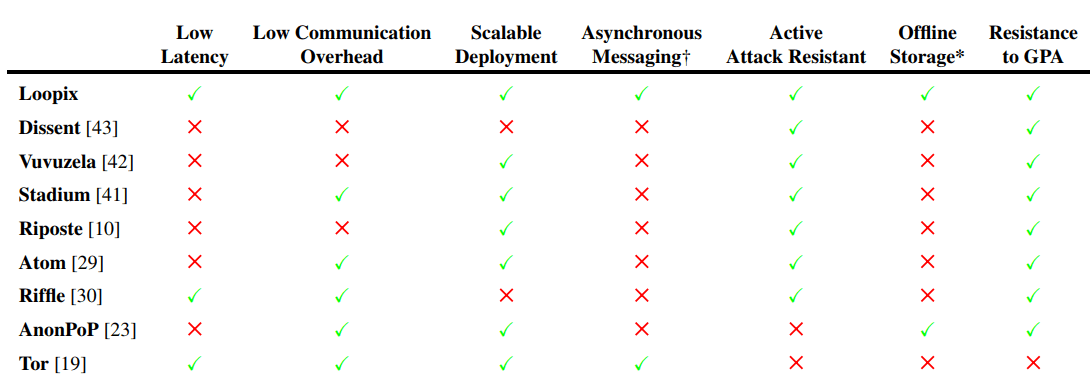
\includegraphics[width=11cm,height=11cm,keepaspectratio]{../yellowpaper/images/state-of-the-art.png}
    \caption{Comparison between anonymous communication systems}
    \label{fig:Comparison between anonymous communication systems}
\end{figure}
\end{comment}

\paragraph{An economic incentive} is what all projects except VPNs and dVPNs
lack which could result in scaling issues and poor performance. Tor and I2P
for example rely on donations and government funding which only covers the cost
of running a node. This has discouraged volunteers to join these networks and the
number of routers in both networks hasn't increased much over the last few years
even though usage and the demand for privacy has risen.
Mixnets are also based on a group of volunteer agents who lack incentives to
participate. Some solutions have proposed adding digital coins to messages, such
that each volunteer can extract only the digital coin designated as a payment
for them. However, malicious volunteers can sabotage the system by extracting
and using their coins without performing their task which consists of forwarding
anonymized messages since there is no verification whether the message arrives
to its final destination or not. Bandwidth providers in dVPNs share their
resources and are granted tokens accordingly as way of payment for their
services. E.g. Mysterium \cite{mysterium}, an open source dVPN built upon a P2P
architecture, uses a smart contract on top of Ethereum to make sure
that the VPN service is paid for adequately.

\subsubsection{Scalability Layer 2 Protocols}
\label{sec:l2protocols}

Blockchain technology (mostly public blockchains like Bitcoin and Ethereum) suffers from a major scalability issue which is due to the fact that every node in the network needs to process every transaction, validate it and stores a copy of the entire state. The number of transactions Ethereum can process for example cannot exceed that of a single node which is currently 15 transactions per second.
\\~\\There have been multiple solutions proposed to treat the scalability issue such as sharding and off-chain computation. Both of these solutions intend to create a second layer of computation in order to reduce the load on the blockchain mainnet.
\\Off chain solutions like Plasma \cite{plasma}, Truebit \cite{truebit} and state channels process transactions outside the Blockchain while still guaranteeing a sufficient level of security and finality. State channels are better known as "payment channels". In models like the "Lightning Network" \cite{lightningnetwork}, a payment channel is opened between two parties by committing a funding transaction, followed by making any number of signed transactions that update the channel's funds without broadcasting those to the blockchain, then closing the channel by broadcasting the final version of the settlement transaction.
Updating the channel balance is done by creating a new set of commitment transactions, then trade revocation keys that render the previous set of commitment transactions unusable. Both parties always have the option to "cash out" by submitting the latest commitment transaction to the blockchain. But if one of them tries to cheat by submitting an outdated commitment transaction, the other party can use the corresponding revocation key to take all the funds in the channel.
\\A channel can no longer be used to route payments from the moment that the close is initiated. There are different closing channel transactions depending on whether both parties agree or disagree to close the channel. If both agree, they provide a digital signature that authorizes this cooperative settlement transaction. In the case where they disagree or only one party is online, a unilateral close is initiated without the cooperation of the other party. This is done by broadcasting a "commitment transaction". Both parties will receive their portion of the money in the channel, but the party that initiates the close must wait a certain delay to receive their money, this delay time is negotiated by the nodes beforehand to receive their funds.
\\The Raiden network is a layer 2 payment solution for the Ethereum blockchain. The project builds off the same technological innovations pioneered by the Bitcoin Lightning Network by facilitating transactions off-chain, but focuses on support for all ERC-20 compliant tokens. Raiden differs in operation from its main chain because it doesn’t require global consensus. However, to preserve the integrity of transactions, Raiden powers token transfers using digital signatures and hash-locks. Referred to as balance proofs, this type of token exchange uses payment channels. Raiden network also introduces a concept called "mediated transfers" which allows nodes to send payments to another node without opening a direct channel to it and those payment channel are updated with absolute amounts and not relative like HOPR (more details in section tickets).
